%%%%
% Modificación de una plantilla de Latex para adaptarla al castellano.
%%%

%%%%%%%%%%%%%%%%%%%%%%%%%%%%%%%%%%%%%%%%%
% Thin Sectioned Essay
% LaTeX Template
% Version 1.0 (3/8/13)
%
% This template has been downloaded from:
% http://www.LaTeXTemplates.com
%
% Original Author:
% Nicolas Diaz (nsdiaz@uc.cl) with extensive modifications by:
% Vel (vel@latextemplates.com)
%
% License:
% CC BY-NC-SA 3.0 (http://creativecommons.org/licenses/by-nc-sa/3.0/)
%
%%%%%%%%%%%%%%%%%%%%%%%%%%%%%%%%%%%%%%%%%

%----------------------------------------------------------------------------------------
%	PACKAGES AND OTHER DOCUMENT CONFIGURATIONS
%----------------------------------------------------------------------------------------

\documentclass[a4paper, 11pt]{article} % Font size (can be 10pt, 11pt or 12pt) and paper size (remove a4paper for US letter paper)

\usepackage[protrusion=true,expansion=true]{microtype} % Better typography
\usepackage{graphicx} % Required for including pictures
\usepackage[usenames,dvipsnames]{color} % Coloring code
\usepackage{wrapfig} % Allows in-line images
\usepackage[utf8]{inputenc}

% Imágenes
\usepackage{graphicx} 

\usepackage{amsmath}
% para importar svg
%\usepackage[generate=all]{svgfig}

% sudo apt-get install texlive-lang-spanish
\usepackage[spanish]{babel} % English language/hyphenation
\selectlanguage{spanish}
% Hay que pelearse con babel-spanish para el alineamiento del punto decimal
\decimalpoint
\usepackage{dcolumn}
\newcolumntype{d}[1]{D{.}{\esperiod}{#1}}
\makeatletter
\addto\shorthandsspanish{\let\esperiod\es@period@code}
\makeatother

\usepackage{longtable}
\usepackage{tabu}
\usepackage{supertabular}

\usepackage{multicol}
\newsavebox\ltmcbox

% Para matrices
\usepackage{amsmath}

% Símbolos matemáticos
\usepackage{amssymb}
\let\oldemptyset\emptyset
\let\emptyset\varnothing

\usepackage[section]{placeins} % Para gráficas en su sección.
\usepackage{mathpazo} % Use the Palatino font
\usepackage[T1]{fontenc} % Required for accented characters
\newenvironment{allintypewriter}{\ttfamily}{\par}
\setlength{\parindent}{0pt}
\parskip=8pt
\linespread{1.05} % Change line spacing here, Palatino benefits from a slight increase by default

\makeatletter
\renewcommand\@biblabel[1]{\textbf{#1.}} % Change the square brackets for each bibliography item from '[1]' to '1.'
\renewcommand{\@listI}{\itemsep=0pt} % Reduce the space between items in the itemize and enumerate environments and the bibliography
\newcommand{\imagen}[2]{\begin{center} \includegraphics[width=90mm]{#1} \\#2 \end{center}}

\renewcommand{\maketitle}{ % Customize the title - do not edit title and author name here, see the TITLE block below
\begin{flushright} % Right align
    {\LARGE\@title} % Increase the font size of the title
    
    \vspace{50pt} % Some vertical space between the title and author name
    
    {\large\@author} % Author name
    \\\@date % Date
    
    \vspace{40pt} % Some vertical space between the author block and abstract
\end{flushright}
}


%Basado en: http://en.wikibooks.org/wiki/LaTeX/Theorems
\usepackage{amsthm}
\newtheorem*{mydef}{Definición}
\newtheorem{mydefn}{Definición}
\newtheorem{theorem}{Teorema}
\everymath{\displaystyle} % Displaystyle por defecto


\usepackage[usenames,dvipsnames]{xcolor}
\definecolor{dkgreen}{rgb}{0,0.35,0}
\definecolor{darkgreen}{rgb}{0,0.35,0}
\definecolor{dkviolet}{rgb}{0.3,0,0.5}
\definecolor{dkred}{rgb}{0.5,0,0}
\definecolor{dkblue}{rgb}{0, 0, 0.9}
\definecolor{darkblue}{rgb}{0, 0, 0.9}
\definecolor{ltblue}{rgb}{0.38, 0.55, 0.8}
\definecolor{maroon}{rgb}{0.5, 0.0, 0.0}
\usepackage{catchfilebetweentags}
\usepackage{verbatim}

% Listings para el código.
\usepackage{listings}
\usepackage{courier}
\lstset{basicstyle=\footnotesize\ttfamily,breaklines=true}
\lstset{frame=tb,aboveskip=3mm,belowskip=3mm,
  aboveskip=3mm,
  belowskip=3mm,
  showstringspaces=false,
  columns=flexible,
  basicstyle={\small\ttfamily},
  numbers=none,
  numberstyle=\tiny\color{gray},
  keywordstyle=\color{blue},
  commentstyle=\color{lgray},
  stringstyle=\color{mauve},
  breaklines=true,
  breakatwhitespace=true
  tabsize=3}
\lstdefinelanguage{XML}
{
  basicstyle=\ttfamily,
  morestring=[s]{"}{"},
  morecomment=[s]{?}{?},
  morecomment=[s]{!--}{--},
  commentstyle=\color{darkgreen},
  moredelim=[s][\color{black}]{>}{<},
  moredelim=[s][\color{red}]{\ }{=},
  stringstyle=\color{blue},
  identifierstyle=\color{maroon}
}


\usepackage[hidelinks]{hyperref}

\newenvironment{coq_example}{\begin{coq}}{\end{coq}}

% Tildes
\lstset{
     literate=%
         {á}{{\'a}}1
         {í}{{\'i}}1
         {é}{{\'e}}1
         {ý}{{\'y}}1
         {ú}{{\'u}}1
         {ó}{{\'o}}1
         {ě}{{\v{e}}}1
         {š}{{\v{s}}}1
         {č}{{\v{c}}}1
         {ř}{{\v{r}}}1
         {ž}{{\v{z}}}1
         {ď}{{\v{d}}}1
         {ť}{{\v{t}}}1
         {ň}{{\v{n}}}1                
         {ů}{{\r{u}}}1
         {Á}{{\'A}}1
         {Í}{{\'I}}1
         {É}{{\'E}}1
         {Ý}{{\'Y}}1
         {Ú}{{\'U}}1
         {Ó}{{\'O}}1
         {Ě}{{\v{E}}}1
         {Š}{{\v{S}}}1
         {Č}{{\v{C}}}1
         {Ř}{{\v{R}}}1
         {Ž}{{\v{Z}}}1
         {Ď}{{\v{D}}}1
         {Ť}{{\v{T}}}1
         {Ň}{{\v{N}}}1                
         {Ů}{{\r{U}}}1    
}

%----------------------------------------------------------------------------------------
%	TITLE
%----------------------------------------------------------------------------------------

\title{\textbf{Seminario 5}\\ % Title
El protocolo XMPP} % Subtitle

\author{\textsc{Ignacio Cordón,\\Mario Román} % Author
\\{\textit{Universidad de Granada}}} % Institution

\date{\today} % Date

%----------------------------------------------------------------------------------------

\begin{document}

\maketitle % Print the title


%----------------------------------------------------------------------------------------
% Escribir una ecuación:
%  \begin{align} 
%  \begin{split}
%----------------------------------------------------------------------------------------

\renewcommand{\abstractname}{Resumen} % Uncomment to change the name of the abstract to something else
\begin{abstract}
\end{abstract}
{\parskip=2pt
\tableofcontents
}
\pagebreak


%--------------------------------------------
% Documento
%--------------------------------------------

\section{Introducción al XMPP}
  El protocolo XMPP (Extensible Messaging and Presence Protocol) se usa para la mensajería
  instantánea, así como para las llamadas de voz y vídeo. El desarrollo del protocolo fue
  iniciado por \textbf{Jeremie Miller} en el 1998, continuado por la comunidad de código abierto Jabber, que dio
  nombre al proyecto, y finalmente formalizado en 2002 por la IETF.\\
  \begin{wrapfigure}{r}{4cm}
  
\includegraphics[width=4cm]{logo.png}
  \end{wrapfigure}
  En 2004 se publicaron los RFCs del protocolo (RFC 3920, RFC 3921, RFC 3922, RFC 3923). Han vuelto a ser actualizados en 2011, y, aunque
  la base del protocolo continúa estable, la \textbf{XMPP Standards Foundation} sigue definiendo extensiones
  al protocolo.
  
  Ha sido adoptado por empresas como Facebook, Tuenti, Whatsapp y Nimbuzz, para su servicio de chat. Asimismo, Google
  también lo adoptó temporalmente en Google Talk, pero lo abandonó en detrimento de su propio protocolo Hangouts.

  En 2003 el protocolo era usado por aproximadamente 10 millones de personas, de acuerdo a los datos de la \textbf{XMPP
  Standards Foundation}	
   
   \subsection{Ventajas}
   \begin{itemize}
     \item \textbf{Descentralización}\\
     La arquitectura de la red XMPP es similar a la de la red email. Cualquiera puede tener su propio servidor XMPP, y
     no existe servidor central
     \item \textbf{Estándar abierto}\\
     La IETF ha formalizado en los RFCS 6120 y 6121 XMPP como un protocolo de mensajería instantánea para el que no es
     necesaria ninguna clase de privilegio para implementar soporte de sus especificaciones. Además su desarrollo no está ligado
     a una única compañía.
     \item \textbf{Seguridad}\\
     Se trata de un protocolo evolucionado y mejorado desde que se creó en 1999. Los servidores XMPP pueden ser aislados
     de la red pública XMPP y los núcleos de las especificaciones XMPP son capaces de proporcionar una alta seguridad
     a través de SASL y TLS.
     
     Cabe destacar que existen múltiples implementaciones del estándar para clientes, servidores, y librerías de código.
     \item \textbf{Flexibilidad}\\
     Las aplicaciones XMPP, más allá de la mensajería instantánea, incluyen funcionalidades como, entre otras: chat de grupo, 
     herramientas colaborativas, compartición de archivos, control de sistemas remotos, geolocalización, VoIP, \ldots
   \end{itemize}
 
   \subsection{Desventajas}
   \begin{itemize}
    \item \textbf{Carece de soporte QoS (Quality of service)}\\
    La garantía de entrega de mensajes debe construirse por encima de la capa XMPP.
    % ? Normally, this is done using simple sequence number attributes in stanzas.
    \item \textbf{Redundancia}\\
    Alrededor del 70\% del tráfico entre servidores son datos de presencia, siendo el 60\% de estos transmisiones 
    redundantes.
    \item \textbf{Escalabilidad}\\
    XMPP adolece del mismo problema de redundancia en sus servicios de chatroom y suscripción. Actualmente se está
    trabajando en su solución.
    \item \textbf{Ausencia de datos binarios}\\
    Al estar basado en XML (transmisión de datos vía texto), la sobrecarga de la red es mayor en comparación 
    con otros protocolos binarios. Este problema ha sido atajado por el \textit{Efficient XML Interchange (EXI) Format},
    en el que XML es fragmentado de forma binaria.
    
    Ahora bien, como los datos binarios deben ser codificados en base64 antes de transmitirse de manera in-band,
    cualquier cantidad considerable de datos binarios (transferencia de archivos) debe ser transmitida out-of-band,
    empleando mensajes in-band para coordinarla. El mejor ejemplo de esto es Jingle, un protocolo de extensión de XMPP
    que añade control de sesiones P2P para VoIP o comunicaciones de videoconferencia.
    
   \end{itemize}


\section{Estructura del XMPP}
  XMPP sigue una arquitectura distribuida cliente/servidor. El cliente y el servidor se comunican a través 
  de una conexión prolongada, normalmente TCP, en el puerto 5222, mediante el intercambio de XML stanzas. Y la información 
  que se envía sobre XMPP va contenida en un streaming de objetos XML. Cuando la comunicación es servidor-servidor la 
  conexión se realiza típicamente a través del puerto 5269, mediante protocolo TCP.  
  
  
  \subsection{Jabber ID y servidores}
    Todo usuario de una red XMPP posee un único Jabber ID (JID), que está estructurado como una dirección email, es decir, 
    consta de usuario y dirección DNS (o en su defecto, dirección IP) del servidor donde el usuario reside, de la forma:
    \texttt{username@example.com}. Así se evita tener que mantener un servidor central con la lista de IDs.
    
    Para posibilitar la conexión de los usuarios desde varios clientes, los JID incluyen una cadena al final, separada
    del ID por una barra /, y conocida como recurso (home, mobile,\ldots). Además, cada recurso puede
    tener asignada una prioridad numérica de manera que \texttt{username@example.com} (bare JID) tenga por ejemplo mayor prioridad que 
    \texttt{username@example.com/mobile}(full JID) y los mensajes enviados al primer JID se entreguen a todos los clientes,
    pero los enviados al segundo JID se entreguen sólo al cliente móvil. Mayor prioridad se refleja en un número más alto.
    
    Asimismo, los JIDs sin la parte del nombre de usuario son también válidos, y pueden ser empleados para mensajes del
    sistema y control de ciertos aspectos en el servidor. Estos JIDs también pueden incluir la parte del recurso.
    
    Un servidor (\texttt{@example.com}) es una entidad que debe ser capaz de:
    \begin{itemize}
     \item Intercambiar XML streams con los clientes conectados y enviar XML stanzas sobre los streams negociados. Así, el
     seridor debe asegurarse de que el cliente se identifica antes de proporcionarle acceso a la red XMPP.
     \item Intercambiar XML streams con otros servidores, y enviar XML stanzas a dichos servidores de acuerdo a la política
     de comunicación que sigan cada uno
     \item Almacenar data usada por los clientes (listas de contactos, información de presencia, \ldots). Esto es una
     responsabilidad secundaria
     \item Hacer de hosting a servicios añadidos al XMPP como la conferencia multi-usuario.
    \end{itemize}
    
      % Imagen de ejemplo de la red
      \begin{center}
      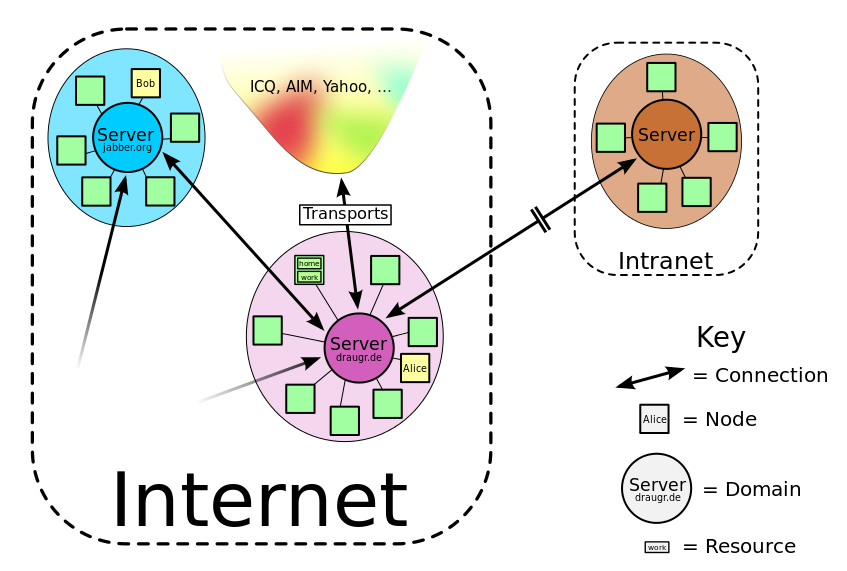
\includegraphics[width=12cm]{network.png}
      \end{center}
      
    
    %? The means to route messages based on a logical endpoint identifier - the JID, instead of by an explicit IP Address 
    % present opportunities to use XMPP as an Overlay network implementation on top of different underlay networks.
  \subsection{XML Stanzas}
    Un cliente y un servidor de XMPP, tras terminar la conexión y la negociación de seguridad,
    pasan a enviarse XML Stanzas, la máxima unidad semántica dentro de \texttt{<stream>} que deben procesar.
    Cada stanza estará iniciada por una etiqueta al primer nivel de profundidad sobre \texttt{<stream>},
    y se finalizará con otra etiqueta al mismo nivel.
    
    El protocolo XMPP usa tres tipos de stanzas, que se describen a continuación: \texttt{<message>}, \texttt{<presence>}
    e \texttt{<iq>}.
  
  \subsection{Tipo de mensajes}
    En los mensajes se puede incluir, aunque no es obligatorio, un atributo que indique el tipo, con objetivo de poder
    presentar las comunicaciones de forma más amigable al usuario, por ejemplo, en un GUI. Si se incluye dicho tipo, debe
    tener uno de los siguientes valores:
    \begin{itemize}
     \item \texttt{chat} El mensaje está enviado en un contexto de conversación uno a uno.
     \item \texttt{error} Un error ha ocurrido en relación a un mensaje previo enviado por el sender.
     \item \texttt{groupchat} Mensaje enviado en el contexto de una conversación multiusuario.
     \item \texttt{headline} El mensaje está generado por un servicio automático que entrega contenido RSS, noticias, 
     deportes, \ldots. No se espera respuesta por parte del receptor.
     \item \texttt{normal} Mensaje enviado en un contexto distinto a conversación uno a uno o multiusuario, que espera
     respuesta por parte del receptor.
    \end{itemize}
    Una aplicación IM debería poder soportar todos estos tipos de mensajes. Si la aplicación recibe un mensaje sin tipificar,
    debe considerar por defecto el tipo \texttt{normal}  
  
  \subsection{Elementos de un mensaje}
    Los mensajes pueden contener elementos como:
    \begin{enumerate}
     \item \texttt{<subject/>}\\
     Contiene caracteres XML human-readable. Especifica el tópico del mensaje. No debe contener atributos, con excepción
     del \texttt{xml:lang}
     \item \texttt{<body/>}
     Contiene XML human-readable. Especifica el contenido del mensaje. No debe contener atributos, con excepción
     del \texttt{xml:lang}
     \item \texttt{<thread/>}
     Contiene XML no human-readable, indicando un identificador para rastrear un thread de conversación (una sesión de
     mensajería instantánea) entre dos entidades. Su valor es generado por el emisor, y debe ser incluido en todas 
     las respuestas. Si se usa, debe ser único a lo largo de una conversación.
    \end{enumerate}

  \subsection{Presencia}
    Se usan, ya sea por \texttt{jabber:client} o \texttt{jabber:server} para expresar la disponibilidad en red en un
    determinado momento de una entidad. Aunque conocer la disponibilidad de una entidad no es estrictamente
    necesario para el intercambio de mensajes XMPP, sí que facilita la interacción en tiempo real. Se indica 
    mediante \texttt{<presence/>}. Puede tomar distintos tipos, aunque no es obligatorio indicar ninguno de ellos:
    \begin{itemize}
     \item \texttt{unavailable} Indica que la entidad deja de estar disponible para comunicación
     \item \texttt{subscribe} El emisor desea suscribirse a la presencia del destinatario %???????
     \item \texttt{subscribed} El emisor ha permitido al receptor recibir su presencia.
     \item \texttt{unsubscribe} El emisor se está desvinculando de la presencia de una entidad.
     \item \texttt{unsubscribed} La petición de suscripción ha sido rachazada o se ha cancelado una suscripción
     \item \texttt{probe} Petición de la presencia de una entidad
     \item \texttt{error} Relacionado con el proceso de envio de una presencia
    \end{itemize}
    
    Además,la presencia puede incluir los elementos:
    \begin{enumerate}
     \item \texttt{<show/>}\\
     A su vez, puede tomar los valores:
     \begin{itemize}
      \item \texttt{away} 
      \item \texttt{chat} La entidad está activa
      \item \texttt{dnd} (Do not disturb)
      \item \texttt{xa} (Extended away) La entidad se encuentra ausente por un gran periodo de tiempo.
     \end{itemize}
     \item \texttt{<status/>}
     Contiene XML human-readable, especificando disponibilidad, y se usa para complementar el valor de \texttt{<show/>}.
     Por ejemplo: En una reunión.
     \item \texttt{<priority/>}
     Contiene un carácter XML no human-readable que representa un entero entre -128 y +127, y que indica el nivel
     de prioridad de un recurso. Por defecto, si no está indicado, se considera a 0.
    \end{enumerate}

    Ejemplo de información de presencia:
\begin{lstlisting}[language=XML]
<presence xml:lang='en'>
  <show>dnd</show>
  <status>Wooing Juliet</status>
  <status xml:lang='cz'>Ja dvo&#x0159;&#x00ED;m Juliet</status>
</presence>
\end{lstlisting}
  \subsection{IQ}
    Los fragmentos de comunicación IQ proporcionan un mecanismo de petición-respuesta estructurado.
  
  \subsection{Proceso de entrega de mensajes}
    La mayoría de ls aplicaciones XMPP están implementadas con una arquitectura cliente-servidor que requiere que un cliente
    establezca sesión en un servidor con objetivo de iniciar procesos de IM y interactuar con los aspectos de presencia.
    
    La comunicación puede efectuarse entre un cliente y un servidor o  bien puede tratarse de un proceso servidor-servidor.
    La descripción del proceso siguiente se hace para el caso cliente-servidor, siendo análoga para la otra posibilidad, 
    donde el servidor que solicita comunicación desempeñaría el rol de cliente:
  
    \subsubsection{Solicitud de inicio de la sesión}
      La sesión se inicia con la etiqueta \texttt{<stream>} y se finalizará con la etiqueta
      \texttt{</stream>}. Por razones de seguridad, a la apertura de la comunicación le sigue
      negociación por TLS y SASL. Después de la negociación, se abre un nuevo canal de comunicación
      más seguro.
      
      Más detalladamente, para requerir un nuevo inicio de sesión, el cliente envía un paquete para la apertura:
      \begin{lstlisting}[language=XML] 
<stream:stream 
	  xmlns='jabber:client'
	  xmlns:stream='http://etherx.jabber.org/streams'
	  to='example.com' 
	  version='1.0'>
      \end{lstlisting}
      y el servidor responde enviando un stream tag al cliente:
      \begin{lstlisting}[language=XML] 
<stream:stream
	  xmlns='jabber:client'
	  xmlns:stream='http://etherx.jabber.org/streams'
	  id='c2s_123'
	  from='example.com'
	  version='1.0'>
      \end{lstlisting}    
      Donde \texttt{example.com} es la URL del servidor XMPP al que se conecta. El servidor
      enviará un paquete con los requisitos para la negociación TLS o SASL. Si nos encontraramos en un caso de 
      comunicación servidor servidor, la línea \texttt{xmlns='jabber:client'} se vería sustituida por 
      \texttt{xmlns='jabber:server'}, y estos son los dos únicos valores posibles que puede tomar dicho campo.
      \begin{lstlisting}[language=XML]
<stream:features> 
  <starttls xmlns='urn:ietf:params:xml:ns:xmpp-tls'>    
    <required/>  
  </starttls>  
  <mechanisms xmlns='urn:ietf:params:xml:ns:xmpp-sasl'>    
    <mechanism>DIGEST-MD5</mechanism>    
    <mechanism>PLAIN</mechanism>   
    <mechanism>EXTERNAL</mechanism>  
  </mechanisms> 
</stream:features>
      \end{lstlisting}

  \subsubsection{Encriptación y autorización}
    Si el servidor necesita una negociación TLS, el cliente enviará un \texttt{STARTTLS} al servidor:
    \begin{lstlisting}[language=XML]
<starttls xmlns='urn:ietf:params:xml:ns:xmpp-tls'/>    
    \end{lstlisting}
    A lo que el servidor responderá en función de si el TLS está permitido o si causa error, informando en
    este último caso al cliente del fallo en la negociación y cerrando ambos stream y la conexión TCP:
    \begin{lstlisting}[language=XML]
<!-- Aceptado -->
<proceed xmlns='urn:ietf:params:xml:ns:xmpp-tls'/> 
<!-- Error -->
<failure xmlns='urn:ietf:params:xml:ns:xmpp-tls'/> 
</stream:stream>
    \end{lstlisting}
    Cuando es procesada la solicitud TLS, el cliente solicitará una nueva sesión, a la que el servidor
    responderá con la necesidad de una negociación SASL.

    Para la negociación SASL, el cliente debe elegir un método de autenticación entre los disponibles
    (DIGEST-MD5, PLAIN y EXTERNAL). En el caso de autorización más simple (PLAIN), se envía una cadena
    codificada como "\texttt{$\backslash$0User$\backslash$0Pass}". El servidor responderá a esto en 
    función de si acepta o no la petición:
    \begin{lstlisting}[language=XML]
<!-- Aceptado -->
<success xmlns='urn:ietf:params:xml:ns:xmpp-sasl'/>
<!-- Error -->
<failure xmlns='urn:ietf:params:xml:ns:xmpp-sasl'/>
    \end{lstlisting}
    
  \subsubsection{Inicio de sesión}
    Si el servidor soporta sesiones, debe incluir un elemento \texttt{<session/>}, que advierte al cliente del 
    correcto establecimiento de sesión.
    
    El servidor indica al cliente que es necesario que establezca sesión:
\begin{lstlisting}[language=XML]
<stream:stream
    xmlns='jabber:client'
    xmlns:stream='http://etherx.jabber.org/streams'
    id='c2s_345'
    from='example.com'
    version='1.0'>
<stream:features>
  <bind xmlns='urn:ietf:params:xml:ns:xmpp-bind'/>
  <session xmlns='urn:ietf:params:xml:ns:xmpp-session'/>
</stream:features>
\end{lstlisting}

    El cliente solicita sesión al servidor:
\begin{lstlisting}[language=XML]
<iq to='example.com'
    type='set'
    id='sess_1'>
  <session xmlns='urn:ietf:params:xml:ns:xmpp-session'/>
</iq>
\end{lstlisting}

    El servidor informa al cliente que la sesión ha sido creada:
\begin{lstlisting}[language=XML]   
<iq from='example.com'
    type='result'
    id='sess_1'/>
\end{lstlisting}

    o en su defecto, si encuentra un error interno por el que no puede concederle sesión, no puede conectarse porque
    sus credenciales carecen de permiso en el servidor, o el usuario ya ha iniciado sesión en el servidor, debe informar:
\begin{lstlisting}[language=XML]
<iq from='example.com' type='error' id='sess_1'>
  <session xmlns='urn:ietf:params:xml:ns:xmpp-session'/>
  <error type='wait'>
    <internal-server-error
        xmlns='urn:ietf:params:xml:ns:xmpp-stanzas'/>
  </error>
</iq>


<iq from='example.com' type='error' id='sess_1'>
  <session xmlns='urn:ietf:params:xml:ns:xmpp-session'/>
  <error type='auth'>
    <forbidden
        xmlns='urn:ietf:params:xml:ns:xmpp-stanzas'/>
  </error>
</iq>
\end{lstlisting}

    Dependiendo de la implementación del servidor si el usuario ya tenía iniciada sesión, cancelará la sesión antearior
    y concederá nueva sesión (primera alternativa de las listadas a continuación), o informará simplemente de que ya
    dispone de una sesión, y mantendrá ésta, en lugar de conceder la nueva.
    
\begin{lstlisting}[language=XML]
<stream:error>
  <conflict xmlns='urn:ietf:params:xml:ns:xmpp-streams'/>
</stream:error>
</stream:stream>
\end{lstlisting}
\begin{lstlisting}[language=XML]
<iq from='example.com' type='error' id='sess_1'>
  <session xmlns='urn:ietf:params:xml:ns:xmpp-session'/>
  <error type='cancel'>
    <conflict xmlns='urn:ietf:params:xml:ns:xmpp-stanzas'/>
  </error>
</iq>
\end{lstlisting}

    \subsubsection{Intercambio de mensajes}
      Si un mensaje es enviado en respuesta a un mensaje previamente recibido de una dirección de la forma 
      \texttt{user@domain/resource}, el valor de \texttt{to} debería ser de la forma \texttt{<user@domain/resource>}. Si el
      mensaje está enviado fuera del contexto de una sesión de chat, o el emisor tiene constancia que el receptor ya no
      está disponible, debe dirigir el mensaje a \texttt{<user@domain>}
      
      Ejemplo de mensaje con \texttt{subject}:
\begin{lstlisting}[language=XML]  
<message
    to='romeo@example.net'
    from='juliet@example.com/balcony'
    type='chat'
    xml:lang='en'>
  <subject>I implore you!</subject>
  <subject
      xml:lang='cz'>&#x00DA;p&#x011B;nliv&#x011B; prosim!</subject>
  <body>Wherefore art thou, Romeo?</body>
  <body xml:lang='cz'>Pro&#x010D;e&#x017D; jsi ty, Romeo?</body>
</message> 
\end{lstlisting}
  
      Ejemplo de thread de conversación:
\begin{lstlisting}[language=XML]        
<message
    to='romeo@example.net/orchard'
    from='juliet@example.com/balcony'
    type='chat'
    xml:lang='en'>
  <body>Art thou not Romeo, and a Montague?</body>
  <thread>e0ffe42b28561960c6b12b944a092794b9683a38</thread>
</message>

<message
    to='juliet@example.com/balcony'
    from='romeo@example.net/orchard'
    type='chat'
    xml:lang='en'>
  <body>Neither, fair saint, if either thee dislike.</body>
  <thread>e0ffe42b28561960c6b12b944a092794b9683a38</thread>
</message>

<message
    to='romeo@example.net/orchard'
    from='juliet@example.com/balcony'
    type='chat'
    xml:lang='en'>
  <body>How cam'st thou hither, tell me, and wherefore?</body>
  <thread>e0ffe42b28561960c6b12b944a092794b9683a38</thread>
</message>

\end{lstlisting}

      
\section{Conexión a otros protocolos. Pasarelas}
  \subsection{Conexión a otros protocolos}
    Una característica útil de la que se intentó dotar a XMPP desde el inicio
    fue la posibilidad de comunicarse con otros protocolos de mensajería.
    Esto lo consigue mediante portales (XMPP gateways) que permiten al usuario
    hacer uso de otros servicios de mensajería instantánea, SMS o email.
    
    Los portales pueden ofrecerlos los servidores y cualquier usuario puede
    registrarse en ellos. Los propios portales funcionarán como proxies,
    autenticándose en la red no-XMPP y actuando en nombre del usuario.
    El proceso será transparente para el cliente, que seguirá funcionando
    como si se comunicara mediante XMPP.
    
    \begin{center}
      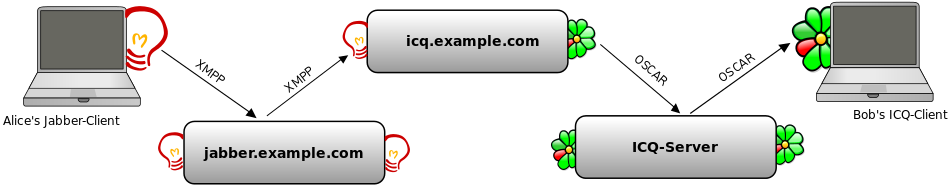
\includegraphics[width=12cm]{external.png}
    \end{center}
    
  \subsection{Protocolos base de XMPP}
  \subsection{Extensiones a XMPP}
  \subsection{XMPP y HTTP}
    La mayoría de firewalls están configurados para permitir el 
    paso de TCP hacia el puerto 80 que usa el protocolo HTML, mientras que
    se bloquea el puerto usado por XMPP.
    
    En las especificaciones originales, XMPP utilizaba las funciones \texttt{GET} y
    \texttt{POST} de HTML para enviar los mensajes al servidor cuando era necesario
    (técnica de polling). Además, existen servidores públicos escuchando conexiones
    XMPP por el puerto 80.

  
%% ------ Bibliografía ------------------------------------------------------
\vfill
\begin{thebibliography}{9}

\bibitem{xmppSF}
  XMPP Standards Foundation. October, 2007.\\
  \url{http://xmpp.org/2007/10/what-is-xmpp/}.
  
\bibitem{xmppWiki}
  XMPP Wikipedia.\\
  \url{http://en.wikipedia.org/wiki/XMPP}
  
\bibitem{xmpp3920}
  RFC 3920.\\
  \url{http://tools.ietf.org/html/rfc3920}
  
\bibitem{xmpp3921}
  RFC 3921.\\
  \url{http://xmpp.org/rfcs/rfc3921.html}
\end{thebibliography}  
  
\end{document}